\begin{frame}[ctb!]
  \frametitle{Cyder Paradigm : Waste Stream Acceptance}
  \begin{figure}[htbp!]
    \begin{center}
      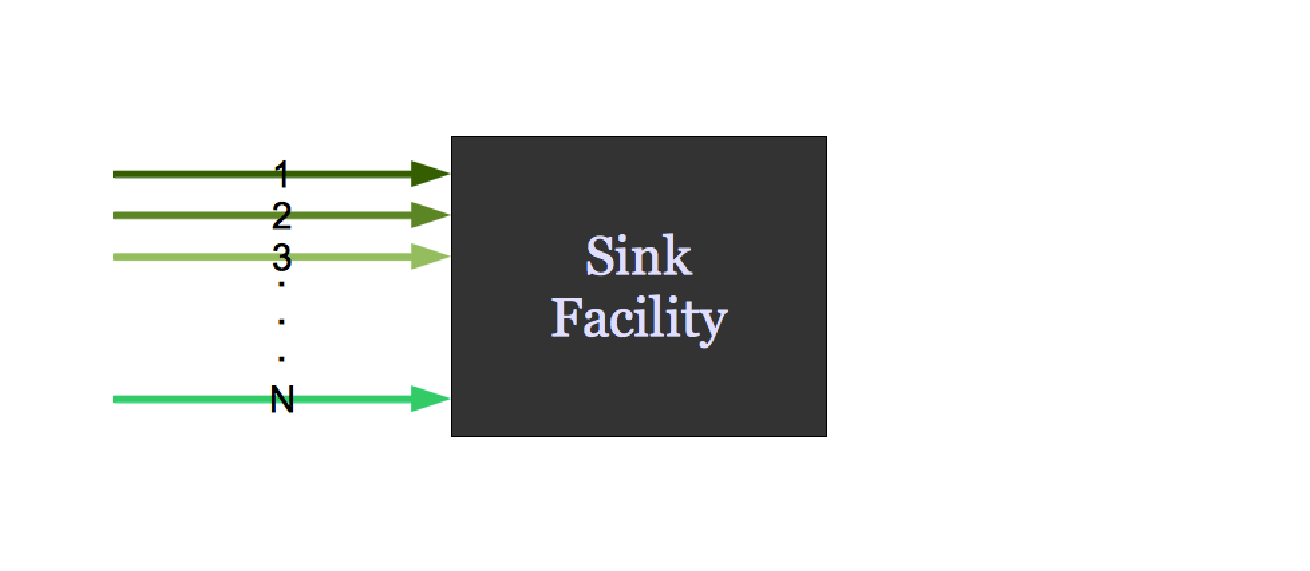
\includegraphics[height=5cm]{./images/sinkfacility.eps}
    \end{center}
    \caption{ To participate in a \Cyclus fuel cycle simulation, \Cyder must 
      accept \textbf{arbitrary} spent fuel and high level waste \textbf{material 
      data objects}.}
    \label{fig:sinkfacility}
  \end{figure}
% Sink Facility ?
\end{frame}

\begin{frame}[ctb!]
  \frametitle{Cyder Paradigm : Waste Stream Conditioning}
  \footnotesize{
  
\begin{figure}[htbp!]
\begin{center}
\def\svgwidth{.5\textwidth}
\input{./images/ws_conditioning.eps_tex}
\end{center}
\caption{In Cyder, discrete waste streams are conditioned into the appropriate 
discrete waste form according to user-specified pairings.}
\label{fig:ws_conditioning}
\end{figure}
}
\end{frame}

\begin{frame}[ctb!]
  \frametitle{Cyder Paradigm : Waste Form Packaging}
  \footnotesize{

\begin{figure}[htbp!]
\begin{center}
\def\svgwidth{.5\textwidth}
\input{./images/wf_packaging.eps_tex}
\end{center}
\caption{In Cyder, one or more waste forms are loaded into the appropriate 
waste package according to user-specified pairings.}
\label{fig:wf_packaging}
\end{figure}
}
\end{frame}

\begin{frame}[ctb!]
  \frametitle{Cyder Paradigm : Waste Package Emplacement}
\footnotesize{
  \begin{columns}[c]
    \column{0.3\linewidth}
Finally, the waste package is \textbf{emplaced} in a buffer component, which 
contains many other waste packages, spaced evenly in a grid. The grid is 
defined by the user input and depends on repository depth, $\Delta z$, waste 
package spacing, $\Delta x$, and tunnel spacing, $\Delta y$ as in Figure 
\ref{fig:repo_layout}.

    \column{0.6\linewidth}
\begin{figure}[htbp!]
\begin{center}
\def\svgwidth{.5\textwidth}
\input{./images/repo_layout.eps_tex}
\end{center}
\caption{The repository layout has a depth and a uniform package spacing.}
\label{fig:repo_layout}
\end{figure}
\end{columns}
  }
\end{frame}


\begin{frame}[ctb!]
  \frametitle{Cyder Paradigm : Modularity }
\begin{figure}[htbp!]
\begin{center}
\def\svgwidth{.6\textwidth}
\input{./images/modularity_layout.eps_tex}
\end{center}
%\caption{}
\label{fig:modularity_layout}
\end{figure}
\end{frame}


\begin{frame}[ctb!]
  \frametitle{Cyder Paradigm : Modularity }
\begin{figure}[htbp!]
\begin{center}
\def\svgwidth{.6\textwidth}
\input{./images/modularity_circle.eps_tex}
\end{center}
%\caption{}
\label{fig:modularity_circle}
\end{figure}
\end{frame}


\begin{frame}[ctb!]
  \frametitle{Cyder Paradigm : Modularity }
\begin{figure}[htbp!]
\begin{center}
\def\svgwidth{.6\textwidth}
\input{./images/modularity_colors.eps_tex}
\end{center}
%\caption{}
\label{fig:modularity_colors}
\end{figure}
\end{frame}


\begin{frame}
  \frametitle{Nested Components}
  Each Component has : 
  \begin{itemize}
    \item a Geometry to describe its dimensions and location
    \item a NuclideModel for contaminant transport 
    \item a ThermalModel for heat transport
    \item a Parent Component at its external barrier
    \item one or more Daughter Components at its internal barrier
  \end{itemize}

  Components have other data members such as a Type (WF, WP, BUFFER, FF), a 
  material data table, a start date, etc. 
\end{frame}
